Raviolimaskin som ska tas fram är tänkt att fylla en Ravioli i tag. Detta görs genom att utforma maskinens degform så att endast en Raviolideg kan placeras på formen. Man ska placera en Raviolideg på maskinens degform. Efter detta ska degformen hissa upp till maskinens pump. Detta görs för att minska avståndet mellan degform och maskinens pump som i sin tur minskar materialslöseriet. I näst ska fyllningsmaterialet pumpas på Raviolidegen som är placerad på formen. Till slut hissas ner degformen och sluter till degformen. Figuren~\ref{blockschema} maskinens olika tillstånd.

\begin{figure}[ht]
	\begin{center}
		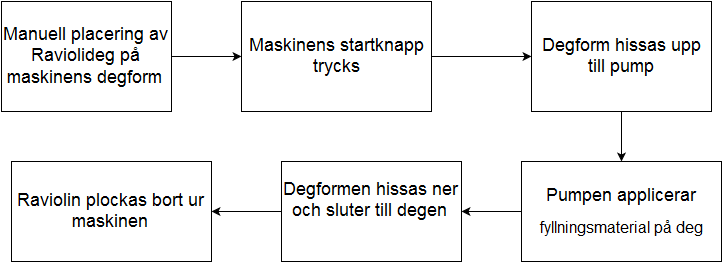
\includegraphics[scale=0.8]{images/blockschema.png}
		\caption{Maskinens olika tillstånd}
		\label{blockschema}	
	\end{center}
\end{figure}
